\documentclass[english,aps,pra,amsmath,amssymb,showpacs,notitlepage,onecolumn]{revtex4-1}
%\usepackage{epsfig}
\usepackage{amsmath}
\usepackage{mathtools}
\usepackage[svgnames]{xcolor}
\usepackage[colorlinks=true, linkcolor=Maroon, urlcolor=Blue]{hyperref} 
%\usepackage{sidecap}
%\usepackage{microtype}
%\usepackage[figuresleft]{rotating}
%\usepackage{caption}
\usepackage{float}
\usepackage{subfigure}
\usepackage{graphicx}
\hypersetup{
  colorlinks,
  citecolor=MidnightBlue,
  linkcolor=DarkRed,
  urlcolor=Blue}
% \usepackage{lscape}
\newcommand{\EssD}{\mathcal{D}}
\def\etal{{\it et al. }}
\def\prb{Phys. Rev. B }
\def\pra{Phys. Rev. A }
\def\prl{Phys. Rev. Lett. }
\def\pla{Phys. Lett. A }
\def\pb{Physica B}
\def\ajp{Am. J. Phys. }
\def\mpl{Mod. Phys. Lett. B }
\def\ijmp{Int. J. Mod. Phys. B}
\def\ijp{Ind. J. Phys. }
\def\ijpap{Ind. J. Pure Appl. Phys. }
\def\ibmjrd{IBM J. Res. Dev. }
\def\pjp{Pramana J. Phys.}

\begin{document}
\title{How to implement a genuine Parrondo's paradox with quantum walks?}
\author{Jishnu Rajendran}
\author{Colin Benjamin}
\email{colin@niser.ac.in}
\affiliation{School of Physical Sciences, National Institute of Science Education \& Research, HBNI, Jatni-752050,\ India }
\begin{abstract}
Parrondo's paradox is ubiquitous in games, ratchets and random walks.The apparent paradox, devised by J.~M.~R.~Parrondo, that two losing games $A$ and $B$ can produce an winning outcome has been adapted in many physical and biological systems to explain their working. However, proposals on demonstrating Parrondo's paradox using quantum walks failed in the asymptotic limits. In this work, we show that instead of a single coin if we consider a two coin initial state which may or may not be entangled, we can observe a genuine Parrondo's paradox with quantum walks. The implications of our results for observing quantum ratchet like behavior using quantum walks is also discussed.   
\end{abstract}
\maketitle
\section{Introduction}
Parrondo's paradox consists of a sequence of games, individually each of which are losing games but provide a winning outcome when played in a deterministic or random order. It has been shown that Parrondo's games have important applications in many physical and biological systems[\onlinecite{control}-\onlinecite{gamethe}]. Quantum version of Parrondo's games were introduced in Refs.[\onlinecite{flitney}-\onlinecite{Meyer}]. Quantum version of the classical random walk on other hand was introduced in 1993 in Ref.[\onlinecite{1993}]. In Refs.[\onlinecite{flitney}-\onlinecite{Meyer}] Parrondo's games are explored using 1-D discrete time quantum walk(DTQW). When a game is played, the net expectation of position of the walker defines a win or a loss. It has been already shown that quantum walk version of Parrondo's paradox does not exist in the asymptotic limits \cite{flitney}-\cite{minli}. The need for studying Parrondo's games via quantum walks is necessitated by the search for applications in building better algorithms\cite{ken} and to explain physical process like quantum ratchets\cite{chandru2}.

\section{Motivation}
Our motivation in this work is to implement a genuine Parrondo's paradox via quantum walk. We show that while previous attempts at implementing Parrondo's paradox with quantum walks failed in asymptotic limits\cite{flitney}-\cite{minli} our method using two coin initial states gives a genuine Parrondo's paradox even in the asymptotic limits.
\\
Parrondo's game as originally introduced in Refs.\cite{Harmer,Parrondo} is a gambling game. A player plays against a bank with a choice of two games $A$ and $B$, whose outcomes are determined by the toss of biased coins. Each of these games is losing when played in isolation but when played alternately or in some other deterministic or random sequence (such as $ABB\ldots, ABAB\ldots$, etc.) can become a winning game. Owing to this counter-intuitive nature, Parrondo's games are also referred to as Parrondo's paradox. The apparent paradox that two losing games $A$ and $B$ can produce a winning outcome when played in an alternating sequence was originally devised by Juan M. R. Parrondo as a pedagogical illustration of the Brownian ratchet\cite{Parrondo}. Parrondo's games have important applications in many physical and biological systems, \emph{e.g.,} in control theory-the random/deterministic combination of two unstable systems can produce a overall stable system\cite{control}.

%\subsection{Game}
The 1-D discrete time quantum walk implementation of Parrondo's paradox is as follows:
Consider two games A and B  alternately played according to time. Game A and B are represented by different quantum operators $U(\alpha_{A},\beta_{A},\gamma_{A})$ and $U(\alpha_{B},\beta_{B},\gamma_{B})$,


\begin{equation}
U(\alpha,\beta,\gamma)=\left(\begin{array}{cc}
e^{i\alpha}\cos\beta & -e^{-i\gamma}\sin\beta\\
e^{i\gamma}\sin\beta & e^{-i\alpha}\cos\beta
\end{array}\right).\label{eq:SU(2)}
\end{equation}
The initial state of the quantum walker is  $\vert\Psi_{0}\rangle=\frac{1}{\sqrt{2}}\vert 0\rangle\otimes(\vert 0\rangle+i\vert 1\rangle),$ where first ket refers to the position space and second ket refers to the single coin space which is initially in  a superposition of heads and tails. The shift in the position space, say from $|n\rangle$ to $|n-1\rangle$ or $|n+1\rangle$, is defined by a unitary operator called shift operator($\mathcal{S}$) defined as,
\begin{equation}
\mathcal{S} =   \sum\limits_{n=-\infty}^{\infty}\vert n+1 \rangle \langle n \vert \otimes \vert 0 \rangle \langle 0 \vert +   \sum\limits_{n=-\infty}^{\infty}\vert n-1 \rangle \langle n \vert \otimes \vert 1 \rangle \langle 1 \vert.
\label{Equ:S}
\end{equation}
 Games \emph{A} and \emph{B} are played alternately in different time steps, i.e., game \emph{A} is played on time steps
$t=nq$ and game \emph{B} is played on time steps $t\neq nq$, where $q$ is the period and $n$ is an integer. The evolution operator can be written as: 
\begin{equation}
U =\left\lbrace 
	\begin{array}{ll}
		\mathcal{S}\cdot U(\alpha_{A},\beta_{A},\gamma_{A})  & \mbox{if } t=nq,n\in Z \\
		\mathcal{S}\cdot U(\alpha_{B},\beta_{B},\gamma_{B}) & \mbox{if } t\neq nq,n\in Z
	\end{array}
\right. 
\end{equation}
and the final state after $N$ steps is given by $\vert\Psi_{N}\rangle=U^{N}\vert\Psi_{0}\rangle$. For $q=3$, it means we play games with the time sequence $ABBABB\ldots$. As denoted in Fig. \ref{fig:win-loss}, after $N$ steps, if the probability $P_{R}$ of the walker to be found to the right of the origin, is greater than the probability $P_{L}$ to be found to the left of the origin, i.e., $P_{R}-P_{L}>0$, we consider the player to win. Similarly, if $P_{R}-P_{L}<0$, the player losses. If $P_{R}-P_{L}=0$, it means the player neither loses nor wins, it's a draw. By making use of the above scheme, Parrondo's games using 1-D DTQW are formulated. We use $P_R-P_L$ to indicate the player win or lose and not expectation value of position because as already shown in Refs.\cite{minli} expectation value may be positive but $P_R-P_L$ may ybe negative this would be an absurd result. The game is constructed with two losing games \emph{A} and \emph{B} having two different biased coin operators $U_{A} (\alpha_{A},\beta_{A},\gamma_{A})$ and $U_{B}(\alpha_{B},\beta_{B},\gamma_{B})$, if we set $\alpha_A=-51,\beta_{A}=45,\gamma_{A}=0,\alpha_{B}=0,\beta_{B}=88,\gamma_B=0$,  $U_{A}^{S}=U^{S}(-51,45,0)$, $U_{B}^{S}=U^{S}(0,88,-16)$ as in Fig.\ref{game}(a). We form a game with sequences \emph{$ABBB\ldots$}. This results in winning at the beginning but in the asymptotic limit the player will lose as in Fig.\ref{game}(b), one can check for different sequences like \emph{$ABAB\ldots ABBABB\ldots$ etc.} and in all cases in the asymptotic limits we lose. Hence Parrondo's paradox does not exist in case of 1-D DTQW. This fact was noted in Refs.~\cite{flitney,minli} also. In particular, Ref.~\cite{flitney} shows with many different sequences like ABAB.., AABAAB.., etc, in asymptotic limits there is no Parrondo's paradox. Hence our motivation to find circumstances for the existence of a genuine Parrondo's paradox in quantum walks. 

\begin{figure}[t]
\centering
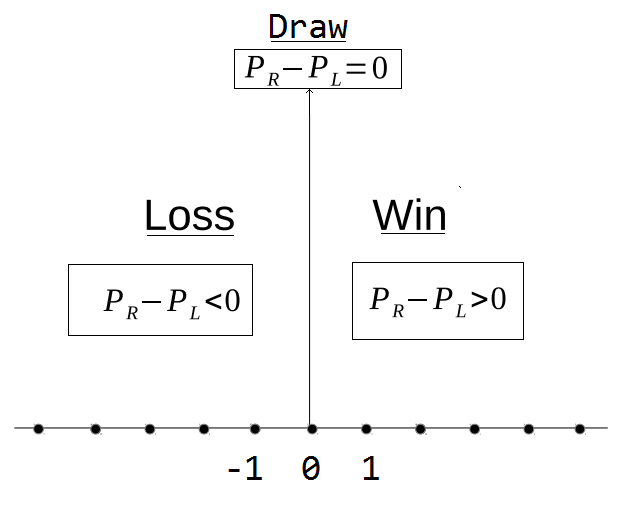
\includegraphics[scale =0.5]{winloss.png}
\caption{Pictorial illustration of the conditions for win or loss for QWs on a line.}
\label{fig:win-loss}
\end{figure}
\begin{figure}[h]
  \centering \subfigure[]{ 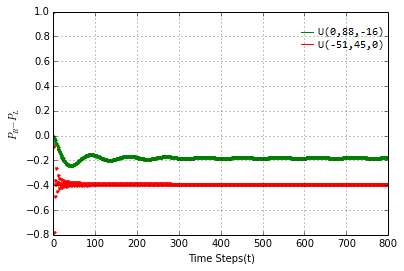
\includegraphics[width=0.43\textwidth]{qwparr.png}}
  \centering \subfigure[]{ 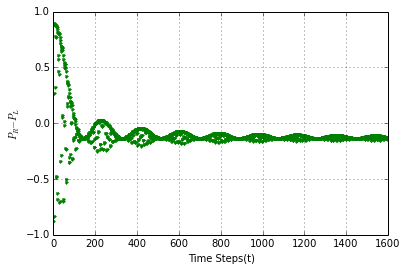
\includegraphics[width=0.43\textwidth]{pd.png}}
\caption{
 a) $P_{R}-P_{L}$ of the walker  after $t$ steps, with initial state $\vert\Psi_{0}\rangle=\frac{1}{\sqrt{2}}\vert 0\rangle\otimes(\vert 0\rangle+i\vert 1\rangle)$, and coin operator $A=U^{S}(-51,45,0)$ (red line) or $B=U^{S}(0,88,-16)$ (green line).  b) $P_{R}-P_{L}$ of the walker with games played in sequence $ABBBABBB\ldots$ (i.e., $q=4$), $A=U^{S}(-51,45,0)$, $B=U^{S}(0,88,-16)$ (1600 steps), herein initially you win($steps < 100$) but in asymptotic limits you lose.
}\label{game}
\end{figure}

\section{Parrondo's paradox using two coin initial state}
As in the previous section, the elements of our two coin quantum walk are the walker, coins, evolution operators for both the coins, walker and a set of observables. The walker is a quantum system with its position denoted as 
$|\text{position}\rangle$ residing in a Hilbert space of infinite but countable dimension ${\cal H}_P$. The basis states $|i \rangle_P$ which span ${\cal H}_P$, and any superposition of the form $\sum_{i} \alpha_i|i\rangle_p$ which are subject to $\sum_i|\alpha_i|^2 = 1$, are valid states for the walker \cite{entangled}. The walker is usually initialized at the \lq origin', i.e., $|\text{position}\rangle_0 = |0\rangle_P$.

The two coin initial state is a quantum system in a 4-D Hilbert space ${\cal H}_{EC}$. We denote the two coin initial state as $|\text{coin}\rangle_0$, which may or may not be entangled-
\begin{equation}\label{e_state}
|\text{coin}\rangle_0 = \cos\left(\frac{\theta}{2}\right) |10\rangle + i \sin\left(\frac{\theta}{2}\right) |01\rangle.
\end{equation}
The initial state of the quantum walker resides in the Hilbert space ${\cal H}_T = {\cal H}_P \otimes {\cal H}_{EC}$ and has the form:
\begin{equation}
|\psi\rangle_0 = |\text{position}\rangle_0 \otimes
|\text{coin}\rangle_0
\end{equation}
which using Eq.\ref{e_state}, gives $|\psi\rangle_0 = |0\rangle \otimes \cos\left(\frac{\theta}{2}\right) |10\rangle + i \sin\left(\frac{\theta}{2}\right) |01\rangle$.
%%%%%%%%%%%%%%%%%%%%%%%%%%%%%%%%%%%%%%%%%%%%%%%%%%%%%%%%%%%%%%%%%%%%%%%%%%%%%%%%%%%
Evolution operators used are unitary as before and since the coin is a bipartite system, the coin is defined as the tensor product of two single-qubit coin operators: $C_{EC}=U_{\alpha_k,\beta_k,\gamma_k}\otimes U_{\alpha_l,\beta_l ,\gamma_l}$, where $k$,$l$ can be any of the Game $A$ and $B$. The evolution operator is fully separable, thus any entanglement in the coins is due to the initial states used. The conditional shift operator $S_{EC}$  allows the walker to move either forward or backward, 
depending on the state of the coin. The operator 
\begin{equation}\label{shift_operator_two_spins}
S_{EC} =  \sum_i |i+1 \rangle_{pp} \langle i| \otimes |00\rangle_{cc} \langle 00|  
+ \sum_i |i\rangle_{pp} \langle i| \otimes |01\rangle_{cc} \langle 01| 
+ \sum_i |i\rangle_{pp} \langle i| \otimes |10\rangle_{cc} \langle 10|
+ \sum_i |i-1 \rangle_{pp} \langle i| \otimes |11\rangle_{cc} \langle 11|
\end{equation}
incorporates the stochastic behavior of the random walk with a two coin initial state. It is only when the coin is in the $|00\rangle$ or $|11\rangle$ state that the walker moves either forward or backward else the walker does not move.
%%%%%% Remember the hat change
The full evolution operator has the structure $U_T = S_{EC}.(I_p \otimes  C_{EC})$ and one can mathematically represent a two coin quantum walk after $N$ steps as $|\psi \rangle_N = (U_T)^N |\psi\rangle_0,$ where $|\psi\rangle_0$ denotes the initial state of the walker and the coins. As defined before, winning and losing in context of Parrondo's game, after $N$ time steps if the probability $P_R$ of the walker to be found to the right of the origin is greater than the probability to be found left of the origin, i.e., $P_R-P_L > 0$ we consider the player to win. However if, $P_R - P_L <  0$ then the player loses and if $P_R-P_L = 0$ it implies a draw. In order to obtain a genuine Parrondo's paradox the two games $A$ and $B$ are now played on the two  coin space as follows: $U_A \otimes U_B$ is operated on the two coins and in the next step $U_B \otimes U_A$ is played on the two coins. Thus, for the first coin we have the series $ABAB\ldots$ while on the second coin we have $BABA\ldots$. The coin operators can as before be defined as-
\begin{equation*}
X=A \otimes B =C_{EC}=U(-51,45,0) \otimes U(0,88,-16)
\end{equation*}
\begin{equation*}
Y=B \otimes A =C'_{EC}=U(0,88,-16) \otimes U(-51,45,0)
\end{equation*}

and are played alternately in time, i.e, in sequence $XYXY\ldots$ and the plot for $P_R -P_L$ as shown in Fig.\ref{result}(a) is obtained. It is evident that the sequence $XYXY\ldots$ provides a winning outcome for two losing games even in asymptotic limits. The fact that individually the sequence $AAA\ldots$ on first coin and $BBB\ldots$ on second coin give a losing outcome can be seen from $P_R-P_L$ plot in Fig.\ref{result}(b).
\begin{figure}[H]
 \centering \subfigure[]{ 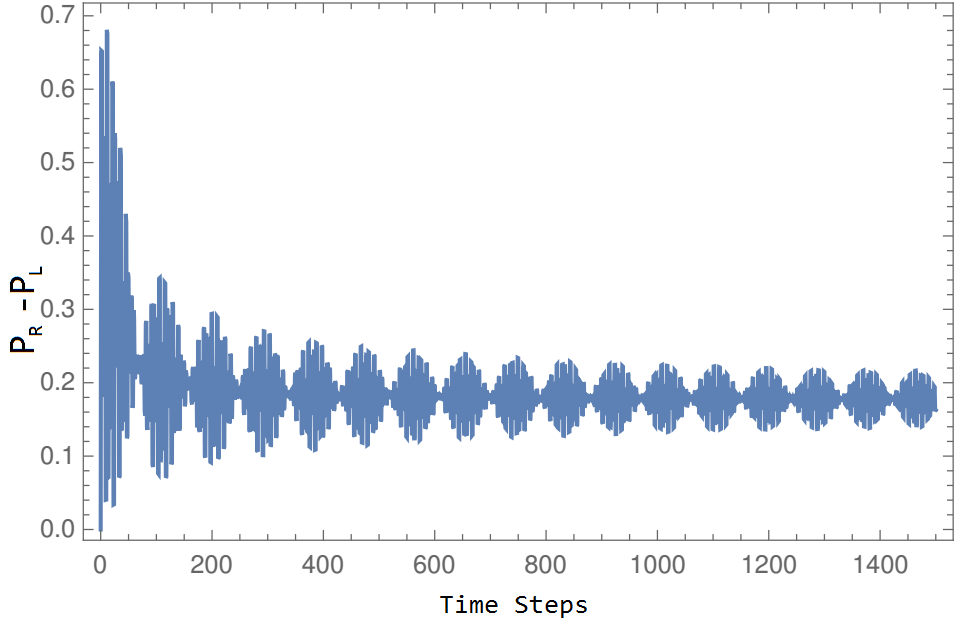
\includegraphics[width=0.33\textwidth]{parr_enta_arbitary-1.png}}
 \centering    \subfigure[]{ 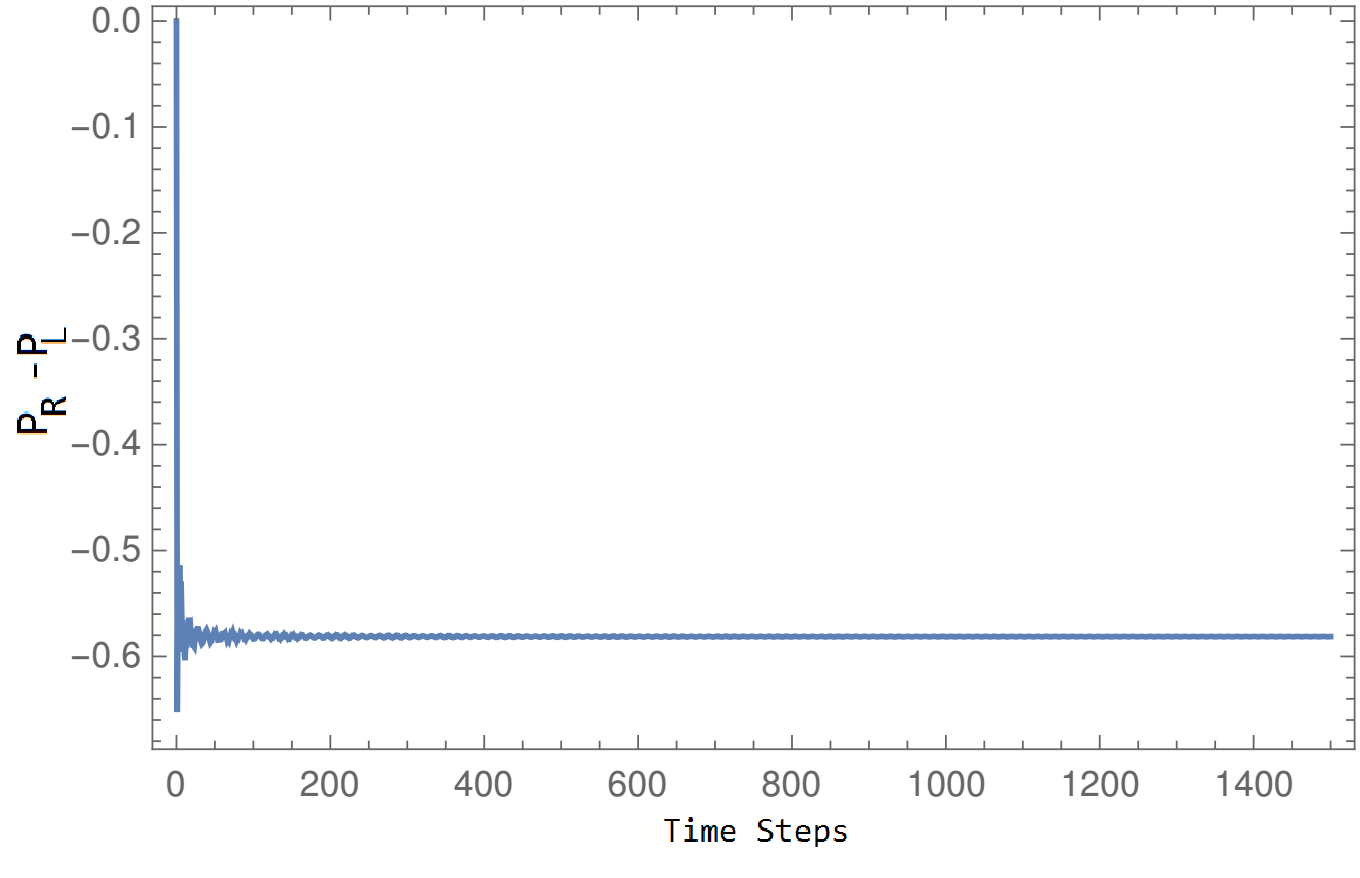
\includegraphics[width=.34\textwidth]{parr_enta_arbitary-2.png}}
 \centering    \subfigure[]{ 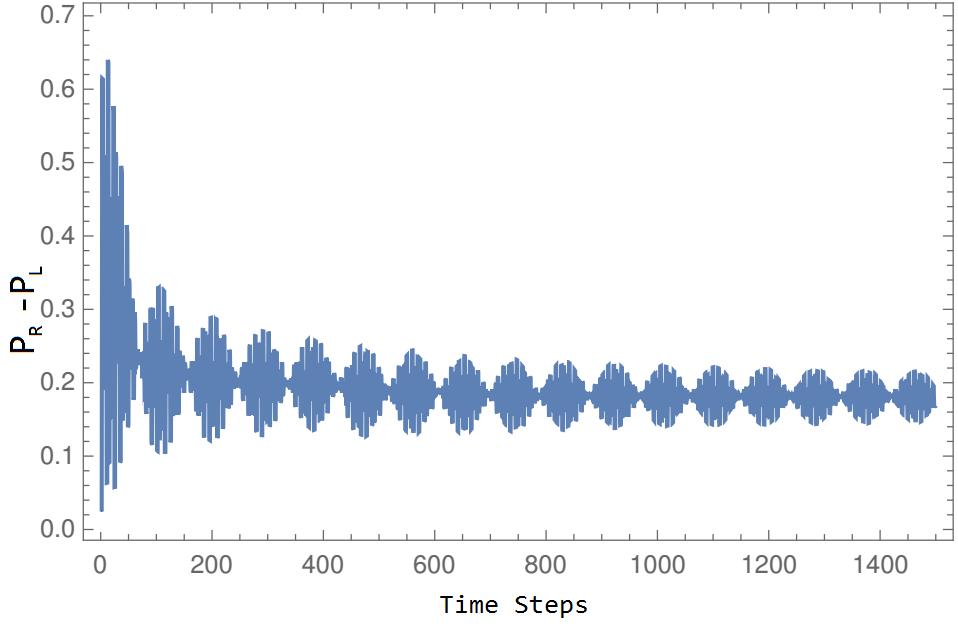
\includegraphics[width=.34\textwidth]{parr_enta_zero.png}}
 \centering    \subfigure[]{ 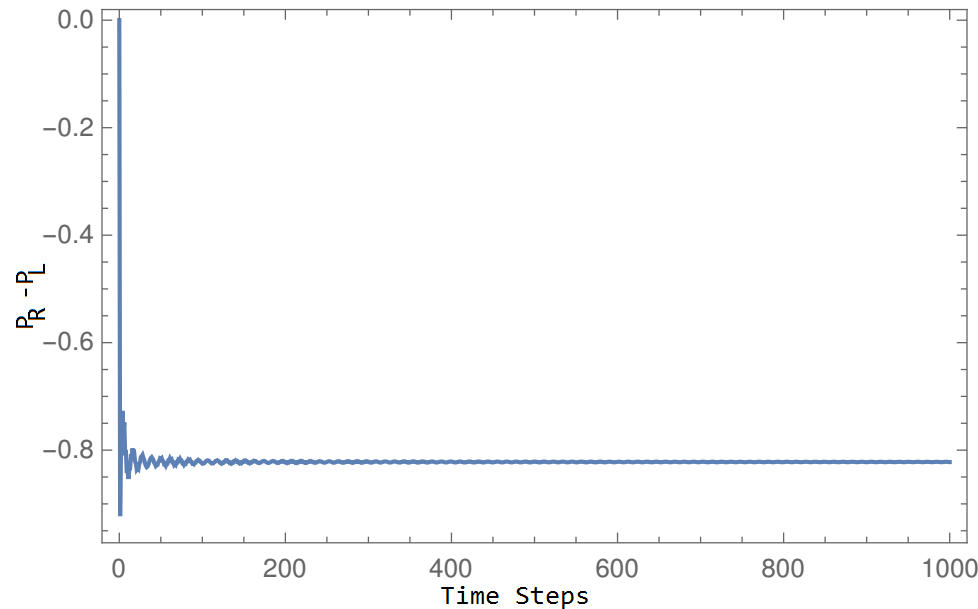
\includegraphics[width=.35\textwidth]{parr_enta_zero1.png}}
 \caption{a) Parrondo walk is evident in the asymptotic limit for partially entangled coin states when $ABAB\ldots$ is played on first coin \& $BABA\ldots$ on second coin. b) However, when $AAAA\ldots$ is played on first \& $BBBB\ldots$ on second coin, one gets a losing outcome.  In c) we show similar to a partially entangled state a non-entangled state also gives a Parrondo's paradox in the asymptotic limit when $ABAB\ldots$ is played on first coin \& $BABA\ldots$ on second coin and finally in d) we show that $P_R-P_L$ is negative in the asymptotic limits when $AAA\ldots$ and $BBB\ldots$ are played on the two coins.}\label{result}
\end{figure}

\section{Discussion}
From Fig. \ref{result} we can conclude that one can obtain a genuine Parrondo's paradox with a non-entangled or a partially entangled two coin state using  quantum walks. When a single coin was considered from Fig.\ref{game} the outcome of Parrondo's games did not give rise to the paradox in the asymptotic limit. In order to obtain a genuine Parrondo's paradox, what is needed is a two-coin state.  
Maximally entangled coins lead to a draw as the probability distribution is perfectly symmetric as noted before in Ref.\cite{entangled}, on the other hand non-entangled or partially entangled coins lead to a Parrondo's paradox. Further, in Fig.~\ref{concur}, we plot the amount of entanglement present in a quantum system, i.e., the concurrence\cite{concurrence}. The concurrence is zero for a separable state and one for a maximally entangled state. Fig.\ref{concur} shows the concurrence for our arbitrary two coin state as a function of $\theta$. One sees that Parrondo's paradox is observed for $0<\theta<\pi/2$ and $3\pi/2<\theta<2\pi$ with the definition as in Fig.~1. In the region $\pi/2 <\theta < 3\pi/2$ there is a role reversal and thus our definition for Parrondo's paradox as used in Fig.~1 is also reversed.
\begin{figure}[h]
\centering 
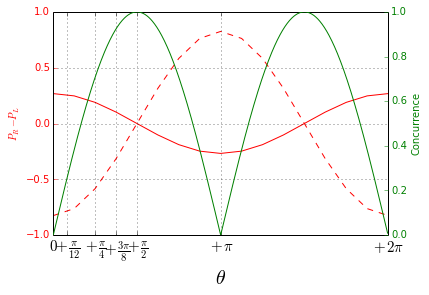
\includegraphics[width=.63\textwidth]{gamma.png}
\caption{Plot of Concurrence(Green), $P_{R}-P_{L}$ (red, solid) for ABAB.. on first coin and BABA...on second coin, and finally $P_{R}-P_{L}$ (red, dashed) for AAAA.. on first coin and BBBB...on second coin. Note that Parrondo's paradox is observed for $0<\theta<\pi/2$ and $3\pi/2<\theta<2\pi$ with the definition as in Fig.~1. In the region $\pi/2 <\theta < 3\pi/2$ there is a role reversal and thus our definition for Parrondo's paradox as used in Fig.~1 is also reversed. }
\label{concur}
\end{figure}


\section{Conclusion}
Our goal in this work was to show evidence of a genuine Parrondo's paradox using quantum walks and we show this using a two coin state. We also considered entanglement between the two coins and showed that maximally entangled states do not show any paradox while non-entangled as well as partially entangled states do show the paradox. Our work can be considered as a demonstration of a  quantum ratchet too, implying particle transport against an applied bias in presence of noise or perturbations. In our case the noise parameter can be considered to reduce entanglement, thus looking at Fig.~\ref{concur}, from zero asymmetry in probability distribution, i.e., non-directed transport, when there is maximal entanglement to finite asymmetry in probability distribution, i.e., directed transport when there is no entanglement, is a clear marker of quantum ratchet like behavior of our system. The quantum ratchet analogies in Parrondo's paradox with quantum walks were also noticed in Ref.~\cite{Meyer}, however without any entanglement. New quantum walks are of great interest to the community as their investigation may lead to new quantum algorithms, which the field search for at present.

\begin{thebibliography}{99}
\bibitem{control} 
A.~Allison and D.~Abbott, Control systems with stochastic feedback, Chaos, Vol. 11, No. 3, pp. 715-724, 2001.

\bibitem{gamethe}
J.~M.~R.~Parrondo and L.~Dinis, Brownian motion and gambling: from ratchets to paradoxical games, Contemporary Physics, Vol 45, pp. 147-157, 2004.

\bibitem{flitney} 
A.~P.~Flitney, Quantum Parrondo's games using quantum walks. arXiv preprint arXiv:1209.2252 (2012).

\bibitem{minli}
M.~Li, Y.~S.~Zhang, G.-C.~Guo, Qunatum Parrondo's games constructed by quantum random walk, arXiv:quant-ph/1303.6831 (2013).

\bibitem{chandru}
C.~M.~Chandrashekar, S.~Banerjee, Parrondoʼs game using a discrete-time quantum walk, Physics Lett. A 375 (2011) 1553.

\bibitem{Meyer}
D.~A.~Meyer, Noisy quantum Parrondo games,Fluctuations and Noise in Photonics and Quantum Optics, Proceedings of SPIE 5111 (2003) 344-350.

\bibitem{1993}
Y.~Aharonov, L.~Davidovich, and N.~Zagury, Quantum random walks, Phys. Rev. A 48, 1687 (1993).

\bibitem{ken} 
V.~Kendon, A random walk approach to quantum algorithms, Phil. Trans. R. Soc. A (2006) 364, 3407-3422. 

\bibitem{chandru2}
S.~Chakraborty, A.~Das, A.~Mallick, C.~M.~Chandrashekar, Quantum ratchet in disordered quantum walk, arXiv:1611.03323.

\bibitem{Harmer} G.~P.~Harmer, D.~Abbott, P.~G.~Taylor and J.~M.~R.~Parrondo, in Proc. 2nd int. Conf. on Unsolved Problems of Noise and Fluctuations (UPoN '99), Adelaide, Australia, \textbf{511}, 189 (1999). %Random Fluctuations: unsolved Problems of Noise.

\bibitem{Parrondo} J.~M.~R.~Parrondo, G.~P.~Harmer, and D.~Abbott, New Paradoxical Games Based on Brownian Ratchets, Phys. Rev. Lett. \textbf{85}, 5226\textendash{}5229 (2000). %New Paradoxical Games Based on Brownian Ratchets.

\bibitem{entangled}
S.~E.~Venegas-Andraca, J.~L.~Ball, K.~Burnett, S.~Bose, Quantum Walks with Entangled Coins, New Journal of Physics 7 (2005) 221, 10.1088/1367-2630/7/1/221.

\bibitem{concurrence}
R.~Hildebrand, Concurrence revisited, Journal of Mathematical Physics, 10.1063/1.2795840 (2007).

\bibitem{blumer}
D.~A.~Meyer and H.~Blumer, Parrondo games as lattice gas automata, Journal of Statistical Physics 107 (2002) 225-239.
\bibitem{package}
Jos\'{e} Luis G\'{o}mez-Mu\~{n}oz and Francisco Delgado, Mathematica add-on for Dirac Bra-Ket Notation, Quantum Algebra and Quantum Computing, http://homepage.cem.itesm.mx/lgomez/quantum/.


\end{thebibliography}
 
\end{document}

